\documentclass{beamer}
\usetheme{Copenhagen}
\setbeamertemplate{navigation symbols}{}
\usepackage[spanish]{babel}
\usepackage{amsmath, amsthm, amssymb}
\usepackage{graphicx}

\begin{document}

\title{Presentación del buscador Moogle!}
\author{Darío Hernández Cubilla C-113}
\date{17 de julio de 2023}
\maketitle

\section{Modelo Vectorial}

\begin{frame}{Modelo Vectorial}

\begin{itemize}
    \item<1-> $ \displaystyle tf(w, d) = \dfrac{frecAbs(w, d)}{palabras(d)}$
    \item<2-> $ \displaystyle idf(w, D) = \ln(\frac{documentos(D)}{ocurrencias(w, D)}) $
    \item <3-> Cada dimensión de un vector de documento d representa una palabra w y su coordenada es $ tf(w, d) * idf(w, D)$ 
    \item<5-> $ \displaystyle \cos{\alpha} = \frac{\vec{q}\cdot\vec{d}}{\left\lvert \vec{q} \right\rvert \left\lvert {\vec{d}} \right\rvert }$
             
\end{itemize}

\only<1>
{
    tf (term frequency) de una palabra w en un documento d es el cociente entre la frecuencia absoluta de w en d
    y la cantidad total de palabras en d, notar que tf(w, D) solo depende del documento en cuestión.
}
\only<2>
{
    idf (inverse document frequency) de una palabra w en una colección de documentos D es el logaritmo
    natural del cociente entre la cantidad total de documentos de D y la cantidad de documentos de D 
    en los que w aparece. Notar que idf(w, D) depende de la colección de documentos.
}

\only<3>
{
    El tf indica la importancia relativa de la palabra sobre el documento, mientras más se repita una
    palabra en un documento, más probable es que este esté relacionado con la palabra
}

\only<4>
{
    El idf indica la rareza de la palabra sobre una colección de documentos, la palabra ''paciente'' es
    mucho más común en una colección de libros de texto de medicina que en una de novelas policíacas, por
    tanto el algoritmo debe darle más importancia en la segunda que en la primera
}

\only<5>
{
    $\vec{q}$ y $\vec{d}$ representan los vectores de tf-idf de la query q y un documento d del corpus,
    $\cos{\alpha}$ es su similitud, nótese que en este espacio n-dimensional, mientras menor sea $\alpha$,
    el ángulo que separa a dichos vectores, menor será su coseno
}

\only<6>
{
    Cada documento (incluyendo a la query) es entonces un vector n-dimensional, donde n es la cantidad
    de palabras únicas en la colección de documentos
}

\end{frame}


\section{Utilidades}

\begin{frame}{Utilidades}
    \begin{itemize}
        \item<1-> Cacheo
        \item<2-> Corrección Ortográfica
        \item<3-> Búsqueda ampliada con sinónimos
        \item<4-> Snippets 
        \item<5-> Operadores
        \begin{itemize}
            \item<6-> Inclusión: \color{blue}{'\^{}'}
            \item<7-> Exclusión: \color{red}{'!'}
            \item<8-> Aumento de importancia: \color{green}{'*'}
        \end{itemize} 
    \end{itemize}

    \only<1>
    {
        De esta forma, suponiendo que la colección de documentos no se modifique, el tiempo de carga
        en ejecuciones subsiguientes a la primera es mucho menor
    }
    \only<2>
    {
        Usando el algoritmo de distancia de Levenshtein, explicado a profundidad en el informe
    }
    \only<3>
    {
        Solo se hace cuando no hay tantos resultados como se esperan, se amplía la búsqueda, se le da
        menos importancia a la búsqueda ampliada, pero complementa los resultados originales
    }
    \only<4>
    {
        Se muestra una parte del documento donde aparezcan algunos elementos de la query, se busca
        que estas palabras aparezcan centradas en esta
    }
    \only<6>
    {
        Hace la existencia de la palabra modificada necesaria en todo documento d para que d aparezca
        en los resultados 
    }
    \only<7>
    {
        Análogo a  '\^{}', pero la palabra debe no existir en d
    }
    \only<8>
    {
        Aumenta exponencialmente el tf de la palabra modificada en el vector de tf-idf de la query
    }
\end{frame}

\section{Comenzar la búsqueda}

\begin{frame}{Búsqueda de Ejemplo}
    \begin{figure}[h]
        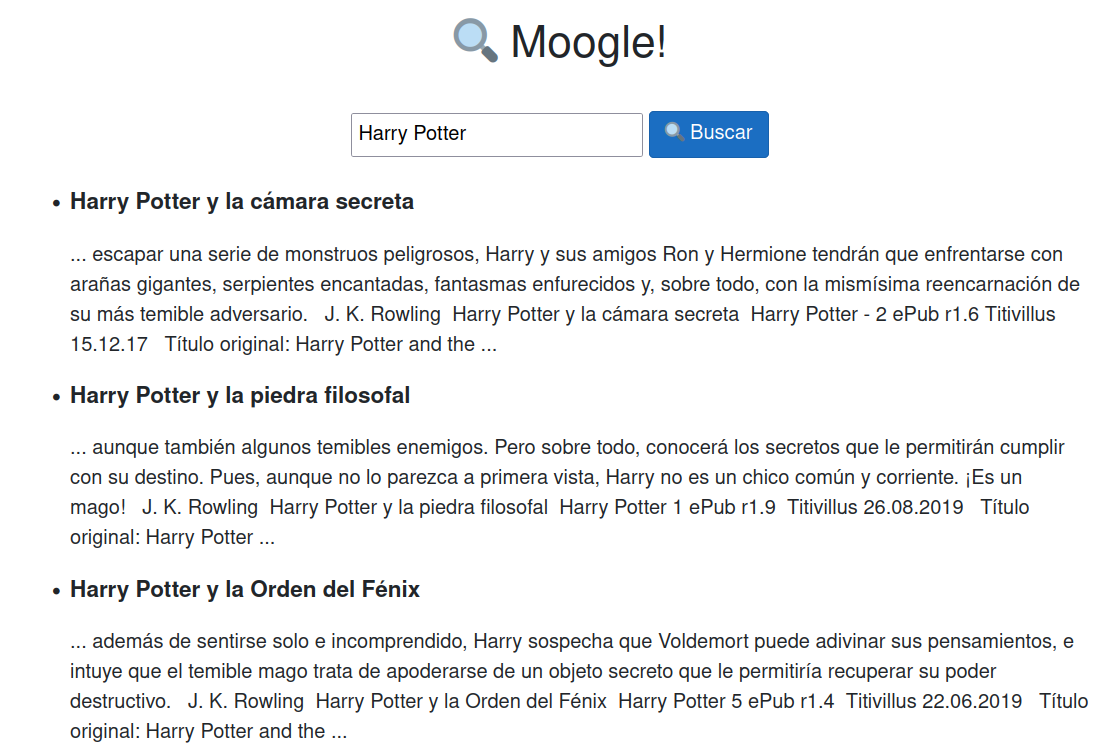
\includegraphics[trim = {0 105  0  0}, clip, width=\textwidth]{sample_search.png}
    \end{figure}
\end{frame}

\section{Operadores}

\begin{frame}{Operador de Exclusión}
    \begin{figure}[h]
        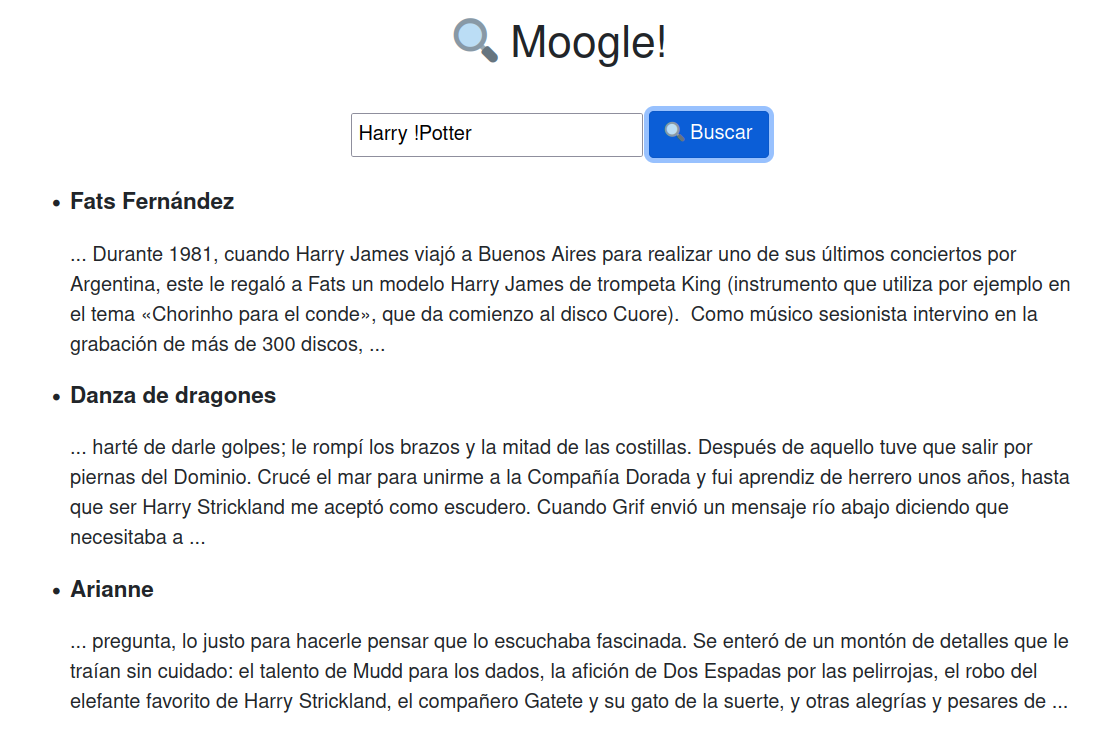
\includegraphics[trim = {0 150  0  0}, clip, width=\textwidth]{exclude1.png}
    \end{figure}
\end{frame}

\begin{frame}{Operador de Inclusión, Original}
    \begin{figure}[h]
        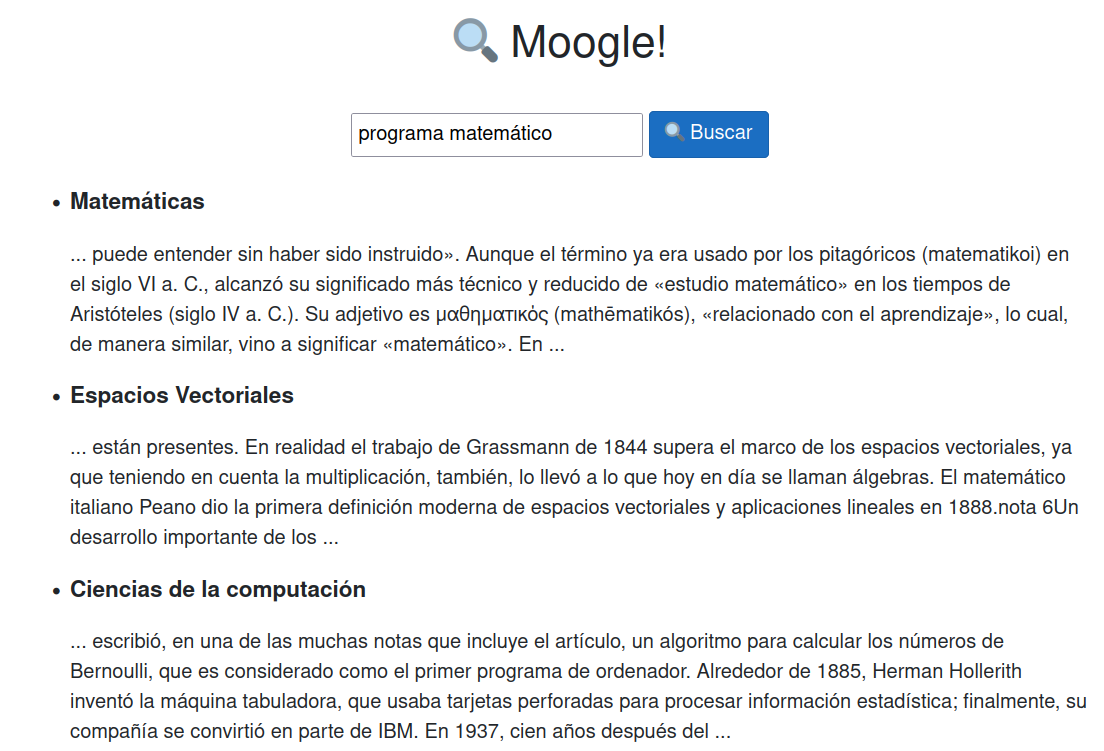
\includegraphics[trim = {0 105  0  0}, clip, width=\textwidth]{include1.png}
    \end{figure}
\end{frame}

\begin{frame}{Operador de Inclusión, Modificado}
    \begin{figure}[h]
        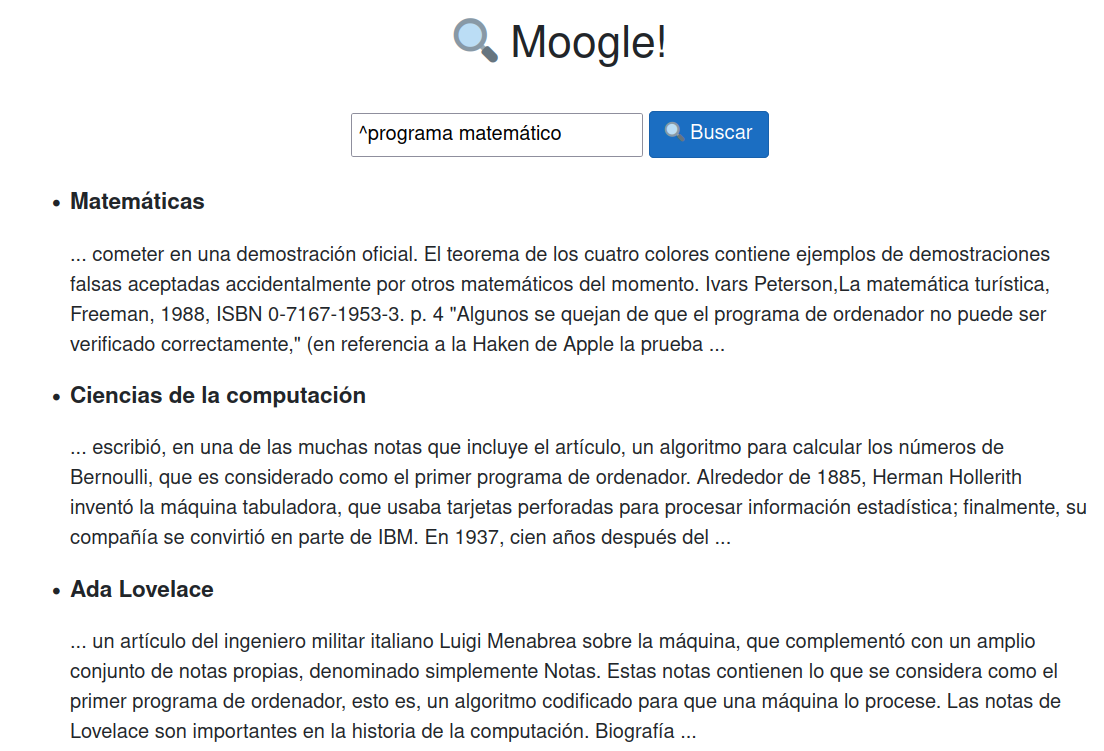
\includegraphics[trim = {0 105  0  0}, clip, width=\textwidth]{include2.png}
    \end{figure}
\end{frame}


\begin{frame}{Operador de aumento de importancia, Original}
    \begin{figure}
        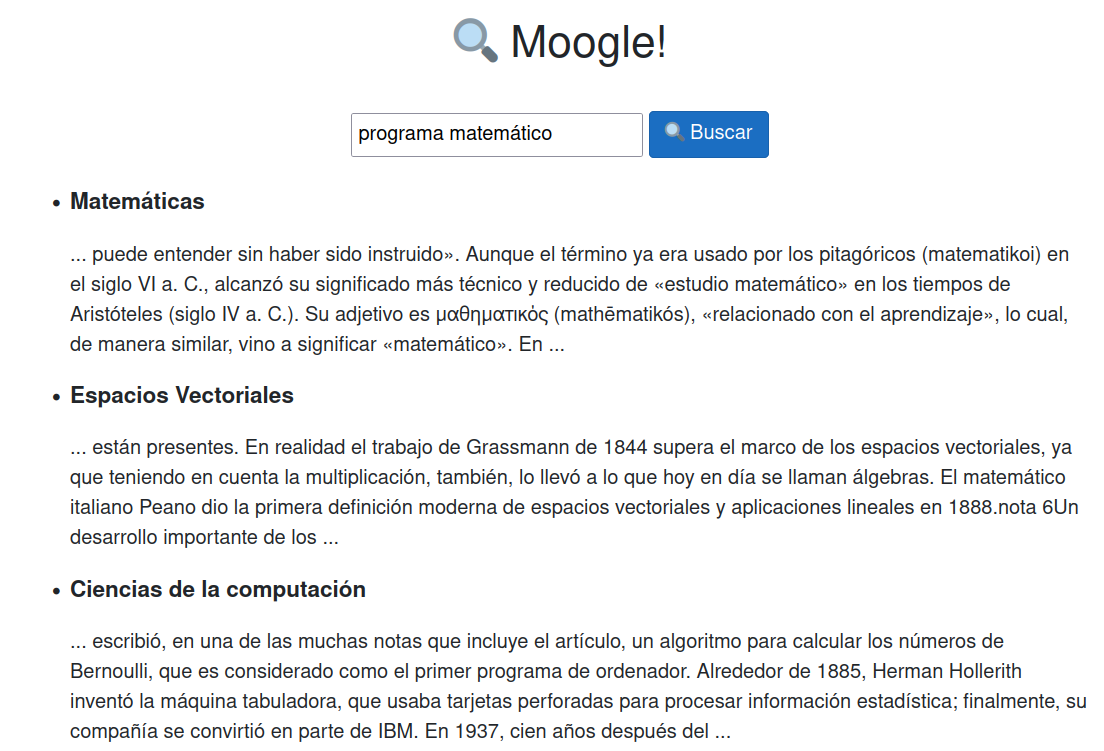
\includegraphics[trim = {0 105  0  0}, clip, width=\textwidth]{include1.png}
    \end{figure}
\end{frame}

\begin{frame}{Operador de aumento de importancia, Modificado}
    \begin{figure}
        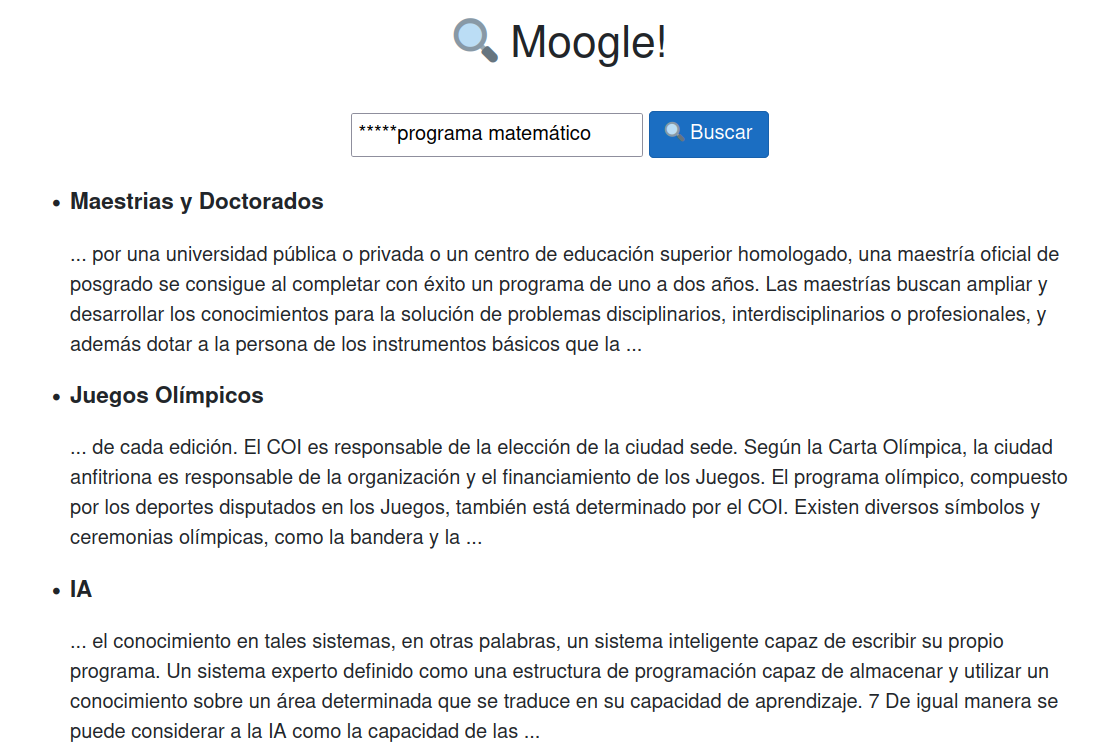
\includegraphics[trim = {0 105  0  0}, clip, width=\textwidth]{asterisk2.png}
    \end{figure}
\end{frame}

\section{Corrección Ortográfica}

\begin{frame}{Corrección Ortográfica}
    \begin{figure}
        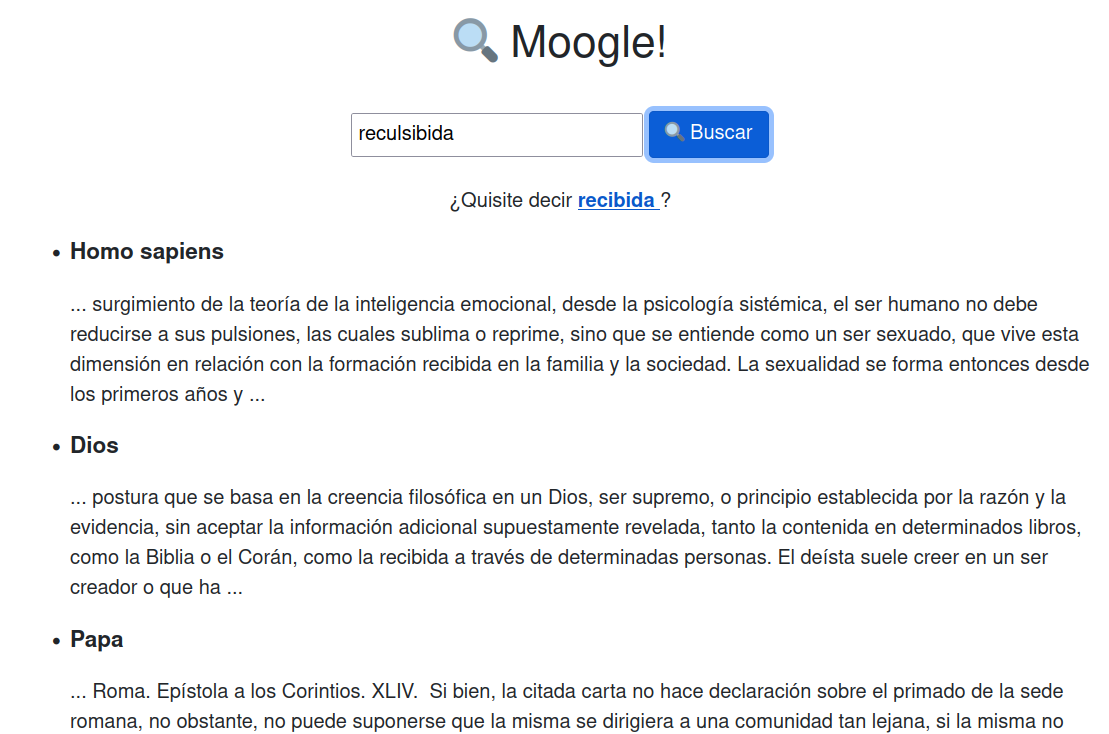
\includegraphics[trim = {0 105  0  0}, clip, width=\textwidth]{correction.png}
    \end{figure}
\end{frame}


\section{Snippet}

\begin{frame}{Snippet}
    \begin{figure}
        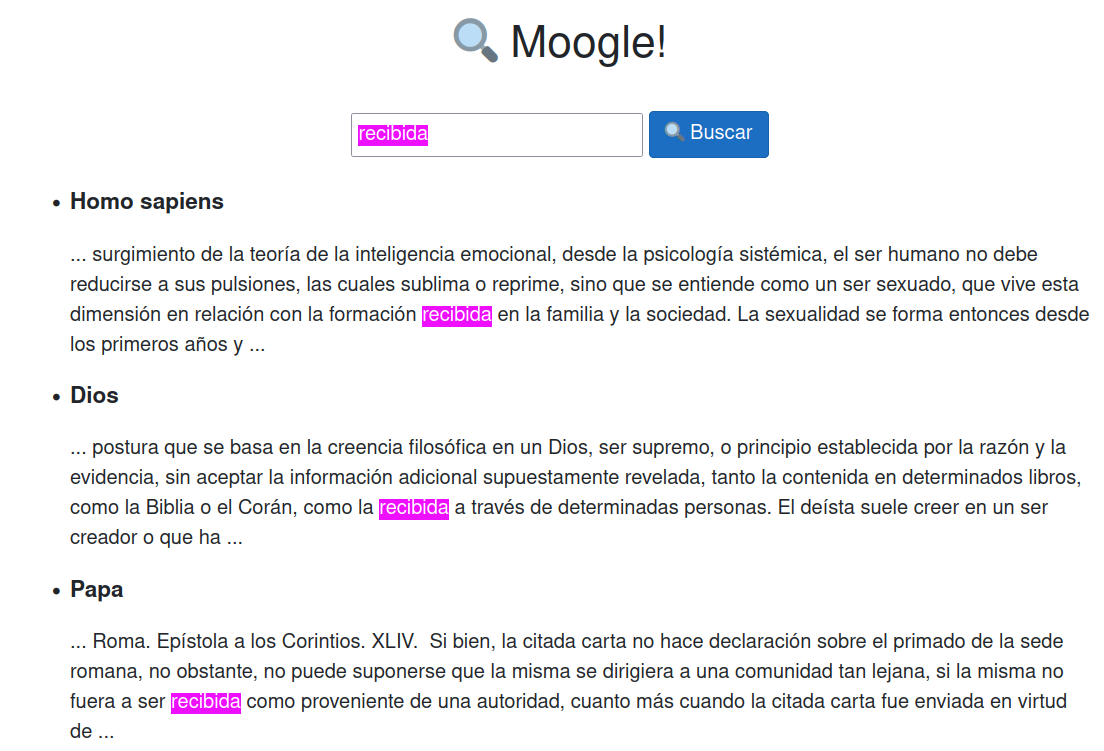
\includegraphics[trim = {0 105  0  0}, clip, width=\textwidth]{snippet.png}
    \end{figure}
\end{frame}



\end{document}

